\documentclass[14pt,a4paper]{scrartcl}
\usepackage{cmap}
\usepackage[utf8]{inputenc}
\usepackage[T1,T2A]{fontenc}
\usepackage[english,russian]{babel}
\usepackage{relsize}
\usepackage{graphicx}
\usepackage{subfigure}
\usepackage{mathtools}
\usepackage{amssymb}
\usepackage{float}
\usepackage{sidecap}
\usepackage{wrapfig}
\usepackage{caption}
\usepackage[table,xcdraw]{xcolor}
\usepackage{minted}
\usepackage{tcolorbox}

\makeatletter
\newenvironment{sqcases}{%
	\matrix@check\sqcases\env@sqcases
}{%
	\endarray\right.%
}
\def\env@sqcases{%
	\let\@ifnextchar\new@ifnextchar
	\left\lbrack
	\def\arraystretch{1.2}%
	\array{@{}l@{\quad}l@{}}%
}
\makeatother

\begin{document}
	\begin{titlepage}
	\begin{center}
		\large
		МИНИСТЕРСТВО НАУКИ И ВЫСШЕГО ОБРАЗОВАНИЯ\\ РОССИЙСКОЙ ФЕДЕРАЦИИ
		
		\vspace{0.5cm}
		
		МГТУ им Н.Э.Баумана
		\vspace{0.25cm}
		
		Факультет ФН
		
		Кафедра вычислительной математики и математической физики
		\vfill
		
		
		Соколов Арсений Андреевич\\
		\vfill
		
		
		{\LARGE Домашнее задания №3 \\ по теории случайных процессов\\[2mm]
		}
		\bigskip
		
		3 курс, группа ФН11-63Б\\
		Вариант 19
	\end{center}
	\vfill
	
	\newlength{\ML}
	\settowidth{\ML}{«\underline{\hspace{0.7cm}}» \underline{\hspace{2cm}}}
	\hfill\begin{minipage}{0.4\textwidth}
		Преподаватель\\
		\underline{\hspace{3cm}} Т.\,В.~Облакова\\
		«\underline{\hspace{0.7cm}}» \underline{\hspace{1.71cm}} 2020 г.
	\end{minipage}%
	\bigskip
	
	
	\vfill
	
	\begin{center}
		Москва, 2020 г.
	\end{center}
\end{titlepage}

\section*{Моделирование гауссовского процесса с данной автоковариационной функцией}
На отрезке $[0,T]$ с шагом $h$ смоделировать $n$ траекторий гауссовского процесса с заданным математическим ожиданием $m(t)$ и заданной автоковариационной функцией $K(t_1,t_2)$. Вывести на печать две-три траектории.\\
Выбрать несколько пар сечений построенного процесса (для далёких значений $t_1$ и $t_2$, для близких, для соседних). Построить для выбранных пар сечений диаграммы рассеяния, вычислить выборочные коэффициенты корреляции, построить $95\%$ доверительные интервалы и сравнить с теоретическими значениями соответствующих коэффициентов корреляции.Сформулировать выводы.\\
\textbf{Начальные данные.}\\
\begin{enumerate}
	\item Интервал -- $[0;10]$\\
	\item Шаг -- $0.05$\\
	\item Число траекторий -- $160$\\
	\item Математическое ожидание -- $m(t) = 1 + {\rm e}^{-t}$\\
	\item Автоковариационная функция -- $K(t_1,t_2) = 2{\rm e}^{-\frac{|t_2 - t_1|}{2}}$ 
\end{enumerate}

\textbf{Решение.}\\
Введём начальные данные:

\begin{minted}{R}
> set.seed(1337)
> Tt <- 10
> Hh <- 0.05
> N <- 160
> Mm <- function(t) {1 + exp(-t)}
> covar <- function(t_1,t_2) {2*exp(-abs(t_2 - t_1)/2)}
\end{minted}

\pagebreak

\subsection*{Моделирование траектории}

Следуя алгоритму предложенному в условии:

\begin{enumerate}
	\item Находим размерность $N+1$ случайного вектора $\xi_0, \xi_h, \ldots, \xi_{Nh}, \quad N = \frac{T}{h}$:
\begin{minted}{R}
# С учётом индекса начала отсчёта:
> Nn <- Tt/Hh
> Nn
[1] 200
\end{minted}

	\item Вычисляем вектор математических ожиданий:
\begin{minted}{R}
> kh <- seq(0,Tt,Hh) # Формуруем равномерную сетку
> head(kh,10)
[1] 0.00 0.05 0.10 0.15 0.20 0.25 0.30 0.35 0.40 0.45

> vect_expected <- Mm(kh) 
> head(vect_expected,5)
[1] 2.000000 1.951229 1.904837 1.860708 1.818731
\end{minted}
	А также матрицу ковариаций:
\begin{minted}{R}
> Sigma_mat <- outer(kh,kh, FUN = covar)
> Sigma_mat[1:5,1:5]
[,1]     [,2]     [,3]     [,4]     [,5]
[1,] 2.000000 1.950620 1.902459 1.855487 1.809675
[2,] 1.950620 2.000000 1.950620 1.902459 1.855487
[3,] 1.902459 1.950620 2.000000 1.950620 1.902459
[4,] 1.855487 1.902459 1.950620 2.000000 1.950620
[5,] 1.809675 1.855487 1.902459 1.950620 2.000000
\end{minted}
	Где элементы $( \sigma_{ij} )$ матрицы $\Sigma$ получены как внешнее произведение вектора сетки на себя (ниже приведено общее определение внешнего произведения)
\begin{equation*}
	\mathbf{u} \otimes \mathbf{v}=\left[\begin{array}{cccc}
	u_{1} v_{1} & u_{1} v_{2} & \dots & u_{1} v_{n} \\
	u_{2} v_{1} & u_{2} v_{2} & \dots & u_{2} v_{n} \\
	\vdots & \vdots & \ddots & \vdots \\
	u_{m} v_{1} & u_{m} v_{2} & \dots & u_{m} v_{n}
	\end{array}\right],
\end{equation*}
	а стандартная операция умножения заменена на автоковариационную функцию.
	\pagebreak
	\item Генерируем с помощью встроенного датчика случайных чисел базовую последовательность независимых стандартных гауссовских случайных величин
	\begin{equation*}
	\overrightarrow{\varepsilon}^T = (\varepsilon_0, \varepsilon_1, \ldots, \varepsilon_N)
	\end{equation*}
	
\begin{minted}{R}
> eps <- rnorm(Nn+1, mean = 0, sd = 1)
> head(eps,5)
[1]  0.1924919 -1.4467018 -0.3231805  1.6222961 -0.6890241
> tail(eps,5)
[1]  0.3135906  0.1310152 -0.9432088  2.9289056  1.1622098
\end{minted}

	\item Представим полученную выше матрицу ковариаций в разложении Холецкого, то есть
	\begin{equation*}
		\Sigma = LL^T
	\end{equation*}

\begin{minted}{R}
L <- t(chol(Sigma_mat))
# Верхние 7*7 элементов, округленные до 4 знаков
> round(L[1:7,1:7],4) 
      [,1]   [,2]   [,3]   [,4]   [,5]   [,6]   [,7]
[1,] 1.4142 0.0000 0.0000 0.0000 0.0000 0.0000 0.0000
[2,] 1.3793 0.3123 0.0000 0.0000 0.0000 0.0000 0.0000
[3,] 1.3452 0.3046 0.3123 0.0000 0.0000 0.0000 0.0000
[4,] 1.3120 0.2971 0.3046 0.3123 0.0000 0.0000 0.0000
[5,] 1.2796 0.2897 0.2971 0.3046 0.3123 0.0000 0.0000
[6,] 1.2480 0.2826 0.2897 0.2971 0.3046 0.3123 0.0000
[7,] 1.2172 0.2756 0.2826 0.2897 0.2971 0.3046 0.3123
\end{minted}
	
	Тогда вектор $\overrightarrow{\eta} = L\overrightarrow{\varepsilon}$ будет иметь многомерное нормальное распределение с нулевым математическим ожиданием и ковариационной матрицей $\Sigma$.

\begin{minted}{R}
> eta <- as.numeric(L %*% eps)
> head(eta,5)
[1]  0.27222466 -0.18632440 -0.28265842  0.23098913  0.01009288
> tail(eta,5)
[1] 1.0266623 1.0422321 0.7219203 1.6188395 1.9418466
\end{minted}
	
	\item Для получения искомого вектора $\overrightarrow{\xi}$ добавляем к каждому элементу $\overrightarrow{\eta}$ соответствующее математическое ожидание $\xi_{kh} = \eta_{k} + m(kh)$:
	
\begin{minted}{R}
> ksi <- vect_expected + eta
> head(ksi,5)
[1] 2.272225 1.764905 1.622179 2.091697 1.828824
> tail(ksi,5)
[1] 2.026718 2.042285 1.721970 2.618887 2.941892
\end{minted}
\end{enumerate}	
\pagebreak

\subsection*{Формирование общего вида функции}	
Описанные в предыдущем пункте действия позволяют смоделировать одну траекторию. Для формирования $N = 160$ траекторий, оформим описанный выше алгоритм в обособленную функцию и реплицируем результат $N$ раз. Тогда функция имеет вид:

\begin{minted}{R}
### Функция моделирования одной траектории
trajectories <- function(Tt, Hh)
{
  Nn <- Tt/Hh
  kh <- seq(0,Tt,Hh)
  vect_expected <- Mm(kh)
  Sigma_mat <- outer(kh,kh, FUN = covar)
  eps <- rnorm(Nn+1, mean = 0, sd = 1)
  L <- t(chol(Sigma_mat))
  eta <- as.numeric(L %*% eps)
  ksi <- vect_expected + eta
  return(ksi)
}
\end{minted}
	
Тогда можем получить лист из $N=160$ траекторий:

\begin{minted}{R}
> traj_list <- replicate(N, trajectories(Tt, Hh), simplify = F)
\end{minted}	

	
Распечатаем несколько траекторий целиком (округлив до 3 знаков после запятой на печати):

\begin{minted}{R}
> round(traj_list[[1]], 3)
[1] 2.272 1.765 1.622 2.092 1.829 2.426 2.667 3.258 3.784
[10] 3.570 3.814 3.205 3.186 3.584 3.484 3.808 3.928 4.095
[19] 4.590 4.321 4.423 4.368 4.029 3.791 3.203 3.699 3.719
[28] 3.880 3.467 3.420 3.749 4.020 3.589 4.597 4.278 4.091
[37] 3.845 3.934 3.521 3.438 4.061 3.428 3.385 3.528 3.240
[46] 3.501 3.634 3.706 3.783 3.494 3.419 3.706 3.419 3.006
[55] 2.764 3.035 2.251 2.403 2.467 2.648 2.176 2.243 2.562
[64] 2.669 2.979 3.141 3.559 4.139 3.857 3.372 3.519 3.387
[73] 3.027 3.035 2.987 3.160 2.871 2.836 3.158 3.057 2.955
[82] 3.362 3.931 3.834 4.187 3.787 3.393 3.061 3.276 3.025
[91] 3.355 2.790 2.724 2.662 2.956 3.261 3.345 3.303 3.207
[100] 3.437 3.442 3.262 3.634 3.619 3.490 3.162 2.856 2.976
[109] 2.949 2.671 2.483 2.235 1.974 2.323 2.409 2.460 2.141
[118] 2.239 2.134 2.441 2.308 2.308 2.107 1.622 1.564 1.954
[127] 1.790 1.574 1.378 0.644 0.451 0.558 0.433 0.316 0.866
[136] 0.997 1.398 1.840 2.788 2.927 2.799 2.471 2.470 2.106
[145] 2.167 2.200 2.092 2.376 2.309 2.966 2.392 2.111 2.269
[154] 2.197 2.612 2.467 2.378 1.912 1.799 1.468 1.336 1.075
[163] 0.802 1.026 0.973 0.738 0.728 0.535 0.498 1.001 1.376
[172] 1.101 1.379 1.368 1.104 1.233 1.403 1.797 1.614 2.069
[181] 2.215 2.153 2.109 1.309 1.098 0.735 1.226 1.363 0.998
[190] 1.201 1.130 1.276 0.814 1.377 1.326 1.952 2.027 2.042
[199] 1.722 2.619 2.942
\end{minted}
	
\begin{minted}{R}
> round(traj_list[[98]], 3)
[1]  2.300  2.050  2.101  2.339  1.822  1.623  1.531  1.049
[9]  1.059  1.225  1.200  1.637  1.926  1.177  1.729  1.638
[17]  1.606  1.356  1.489  1.612  1.946  1.315  1.371  1.600
[25]  1.928  1.862  1.993  2.279  1.774  1.192  0.888  0.928
[33]  1.355  1.566  1.427  0.790  0.914  0.697 -0.068 -0.118
[41] -0.325 -0.338 -0.515 -0.684 -0.860 -0.460 -0.157 -0.620
[49] -0.593 -0.664 -0.373  0.105  0.381  0.791  1.203  1.286
[57]  1.006  0.545  0.347  0.120  0.908  0.778  1.051  0.853
[65]  1.285  1.127  1.106  1.129  1.143  0.597  0.675  0.504
[73]  0.541 -0.137  0.367  0.357  0.516  0.449  0.817  1.325
[81]  1.688  1.611  1.797  1.937  1.153  1.708  1.478  1.240
[89]  1.489  1.174  0.738  0.076 -0.039 -0.029  0.241  0.300
[97]  0.209  0.109  0.032  0.123  0.586  0.719  0.633  0.608
[105]  0.900  1.777  1.837  1.852  1.697  2.312  2.324  2.434
[113]  1.801  1.984  1.538  1.366  1.185  1.249  0.671  1.356
[121]  1.480  1.242  0.931  0.782  0.950  0.613  0.710  0.918
[129]  0.764  0.823  1.149  0.889  1.206  1.136  1.456  1.244
[137]  1.436  0.868  0.751  0.650  0.359  0.480  0.121  0.193
[145]  0.073  0.552  0.425  0.580  0.263 -0.050  0.006 -0.037
[153] -0.094 -0.083  0.085 -0.302 -0.178 -0.574 -0.782 -0.384
[161] -1.190 -1.070 -0.170 -0.609  0.000  0.066  0.394  0.245
[169]  0.072  0.422  0.250  0.232 -0.285 -0.707 -1.422 -1.730
[177] -1.635 -0.937 -1.214 -1.618 -1.135 -1.548 -1.442 -1.148
[185] -1.003 -1.125 -0.979 -0.789 -0.536  0.083 -0.060 -0.494
[193] -0.224 -0.490 -0.303  0.303  0.504  0.481  0.877  1.274
[201]  1.377
\end{minted}

	
\begin{minted}{R}
> round(traj_list[[155]], 3)
[1]  1.085  0.856  0.640  1.093  0.824  0.683  0.967  0.648
[9]  0.669  0.331  0.147  0.294  0.350  0.499  0.233  0.269
[17]  0.318  0.071  0.336  0.496  0.661  0.803  0.375  0.145
[25] -0.134 -0.035 -0.248  0.184  0.161  0.396  0.416  0.997
[33]  1.022  0.840  0.781  0.742  0.769  1.040  0.762  0.670
[41]  0.534  0.514  0.068  0.482  0.055  0.371  0.248  0.458
[49]  0.296  0.014 -0.148 -0.411 -0.136  0.271  0.837  0.615
[57]  0.682  0.788  1.071  0.582  0.127  0.354  0.421  0.641
[65]  0.509  0.749  0.644  0.534  0.239  0.061  0.147 -0.147
[73]  0.016 -0.397 -0.787 -0.521 -0.660 -0.774 -0.706 -0.707
[81] -0.559 -0.622 -0.166 -0.451 -0.750 -0.801 -0.496 -0.636
[89] -0.085  0.308  0.496  0.823  0.514  0.985  0.852  0.647
[97]  0.685  1.105  1.425  1.282  1.377  0.988  1.231  1.275
[105]  1.116  0.940  0.700  0.656  0.585  0.776  0.600  1.015
[113]  0.812  0.507  0.343  0.587  0.759  0.991  0.458  0.030
[121]  0.264  0.071  0.312  0.403  0.237  0.724  0.890  0.918
[129]  0.754  0.354  0.033  0.649  0.571  0.669  0.309 -0.243
[137] -0.353 -0.731 -1.049 -0.980 -1.208 -0.535  0.119  0.484
[145]  0.063  0.032  0.297  0.765  0.661  0.955  0.920  0.615
[153]  0.882  0.842  0.726  0.830  0.932  0.509  0.314  0.534
[161]  0.854  0.839  1.247  1.484  1.439  1.075  0.682 -0.158
[169] -0.023  0.076 -0.481 -0.348 -0.687 -0.489  0.093  0.329
[177]  0.401 -0.018  0.229  0.124  0.142 -0.102  0.122 -0.232
[185]  0.406  0.244  0.053 -0.089 -0.124  0.388  0.269  0.720
[193]  1.234  1.042  1.199  0.900  1.141  0.958  1.474  2.047
[201]  1.912
\end{minted}

\begin{figure}[H]
	\begin{minipage}[h]{1\linewidth}
		\center{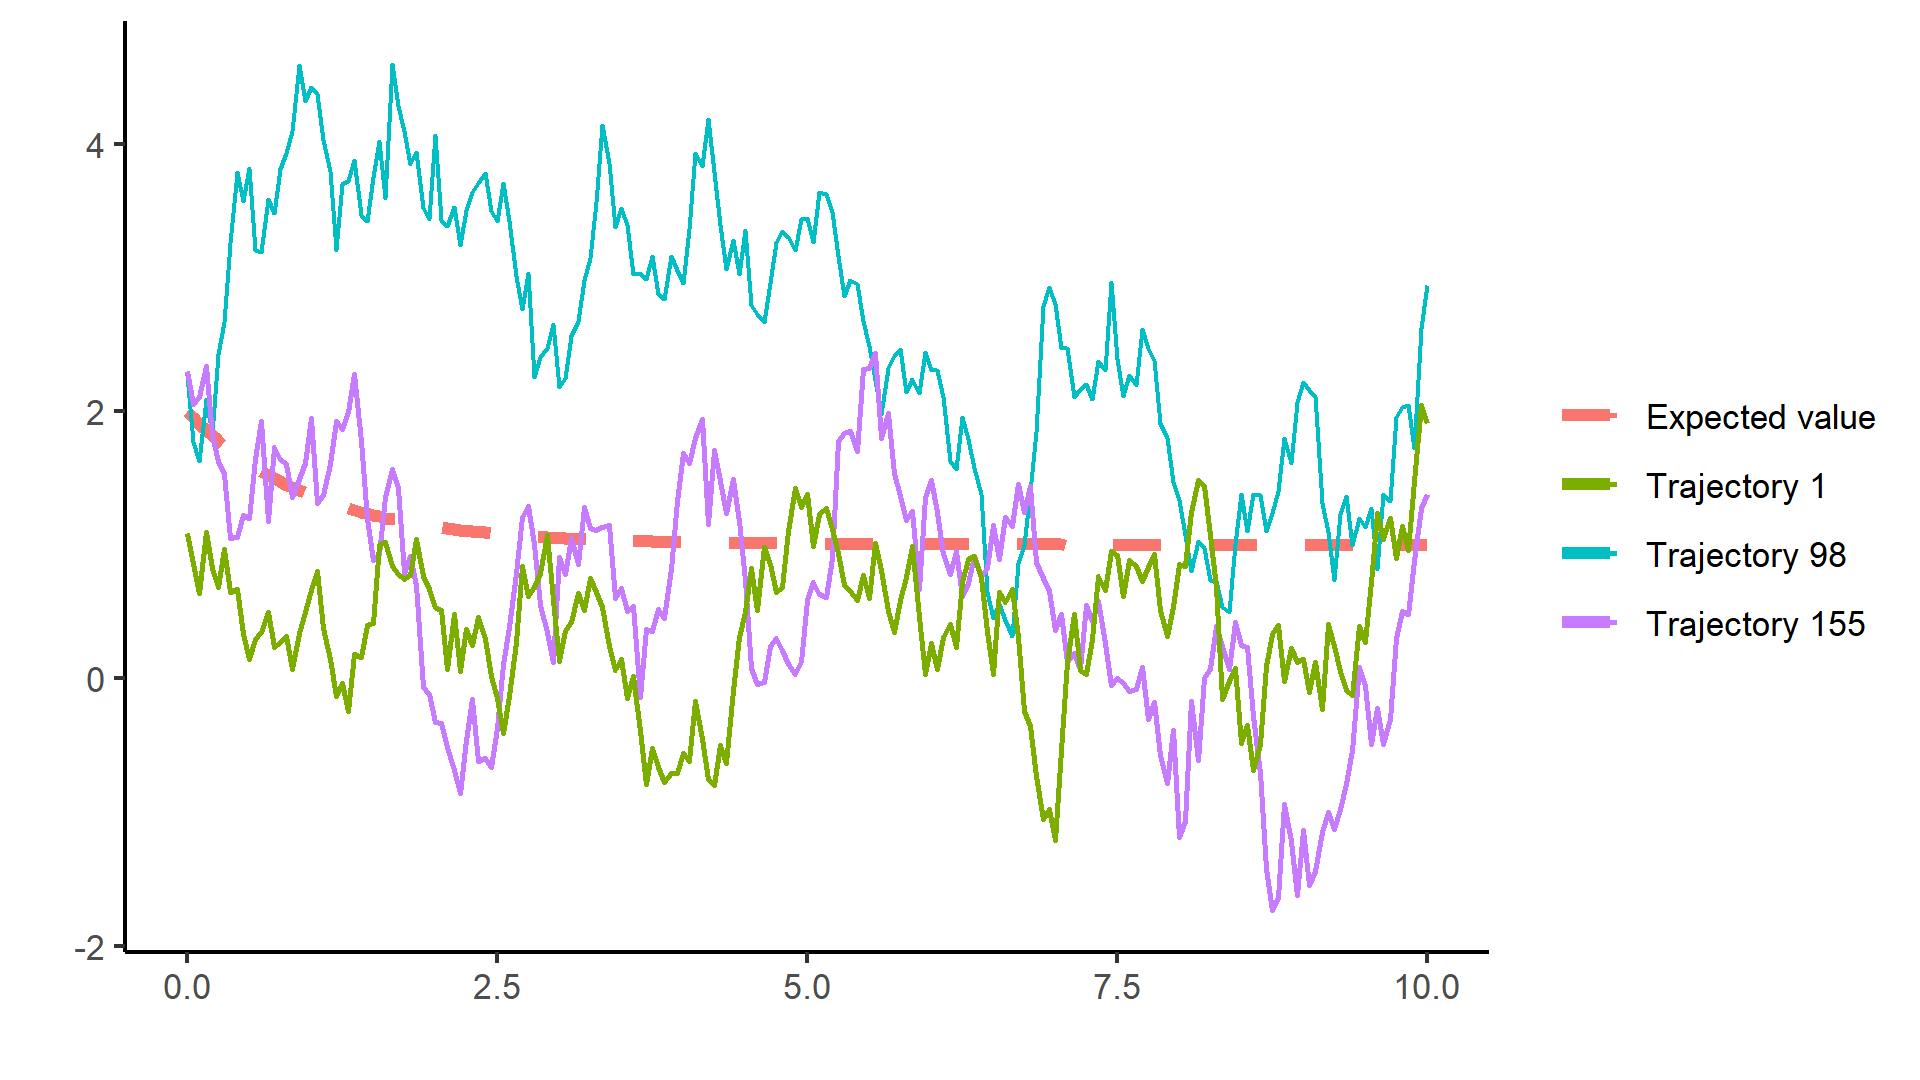
\includegraphics[width=0.95\linewidth]{../img/trajs.png}}  \\
		\caption*{Совмещённые графики трёх траекторий и математического ожидания}
	\end{minipage}
\end{figure}



\pagebreak

\subsection*{Рассмотрение сечений}
Выберем несколько пар сечений (для далёких значений $t_1$ и $t_2$, для близких, для соседних). Рассмотрим такие пары:

\begin{equation*}
		\begin{cases}
			t_1 = 1;\\
			t_2 = 2;
		\end{cases}
		\quad
		\begin{cases}
			t_1 = 20;\\
			t_2 = 150;
		\end{cases}
		\quad
		\begin{cases}
			t_1 = 130;\\
			t_2 = 155;
		\end{cases}
\end{equation*}

Построим для выбранных пар сечений диаграммы рассеяния, вычислим выборочные коэффициенты корреляции и найдём 95\% доверительные интервалы. \\
\subsubsection*{Первый случай: $t_1 = 1, \; t_2 = 2$}
Получим сечение:

\begin{minted}{R}
> t1 <- 1
> t2 <- 2
> selected_cut <- as.data.frame(matrix(c(sapply(traj_list, `[[`, t1),
+                                        sapply(traj_list, `[[`, t2)),
+                                      ncol = 2, byrow = F))
> colnames(selected_cut) <- c("t1","t2")
> head(selected_cut)
	V1        V2
1 2.2722247 1.7649050
2 2.5048647 2.1493222
3 1.1405835 0.7866049
4 1.2777371 1.1495950
5 0.4894897 0.9261547
6 0.3540884 0.8774490
\end{minted}

Построим диаграмму рассеяния для полученной пары сечений:

\begin{minted}{R}
> png(filename = "../img/1.png",
+     width = 1920, height = 1080,
+     res = 96 * 3)
> ggplot(selected_cut, aes(x = t1, y = t2)) + geom_point() +
+   labs(title = "Scatter plot",
+        subtitle = "t1 = 1, t2 = 2",
+        x = "", y = "") + 
+   theme(plot.title = element_text(hjust=0.5))
> dev.off()
\end{minted}

\begin{figure}[H]
	\begin{minipage}[h]{1\linewidth}
		\center{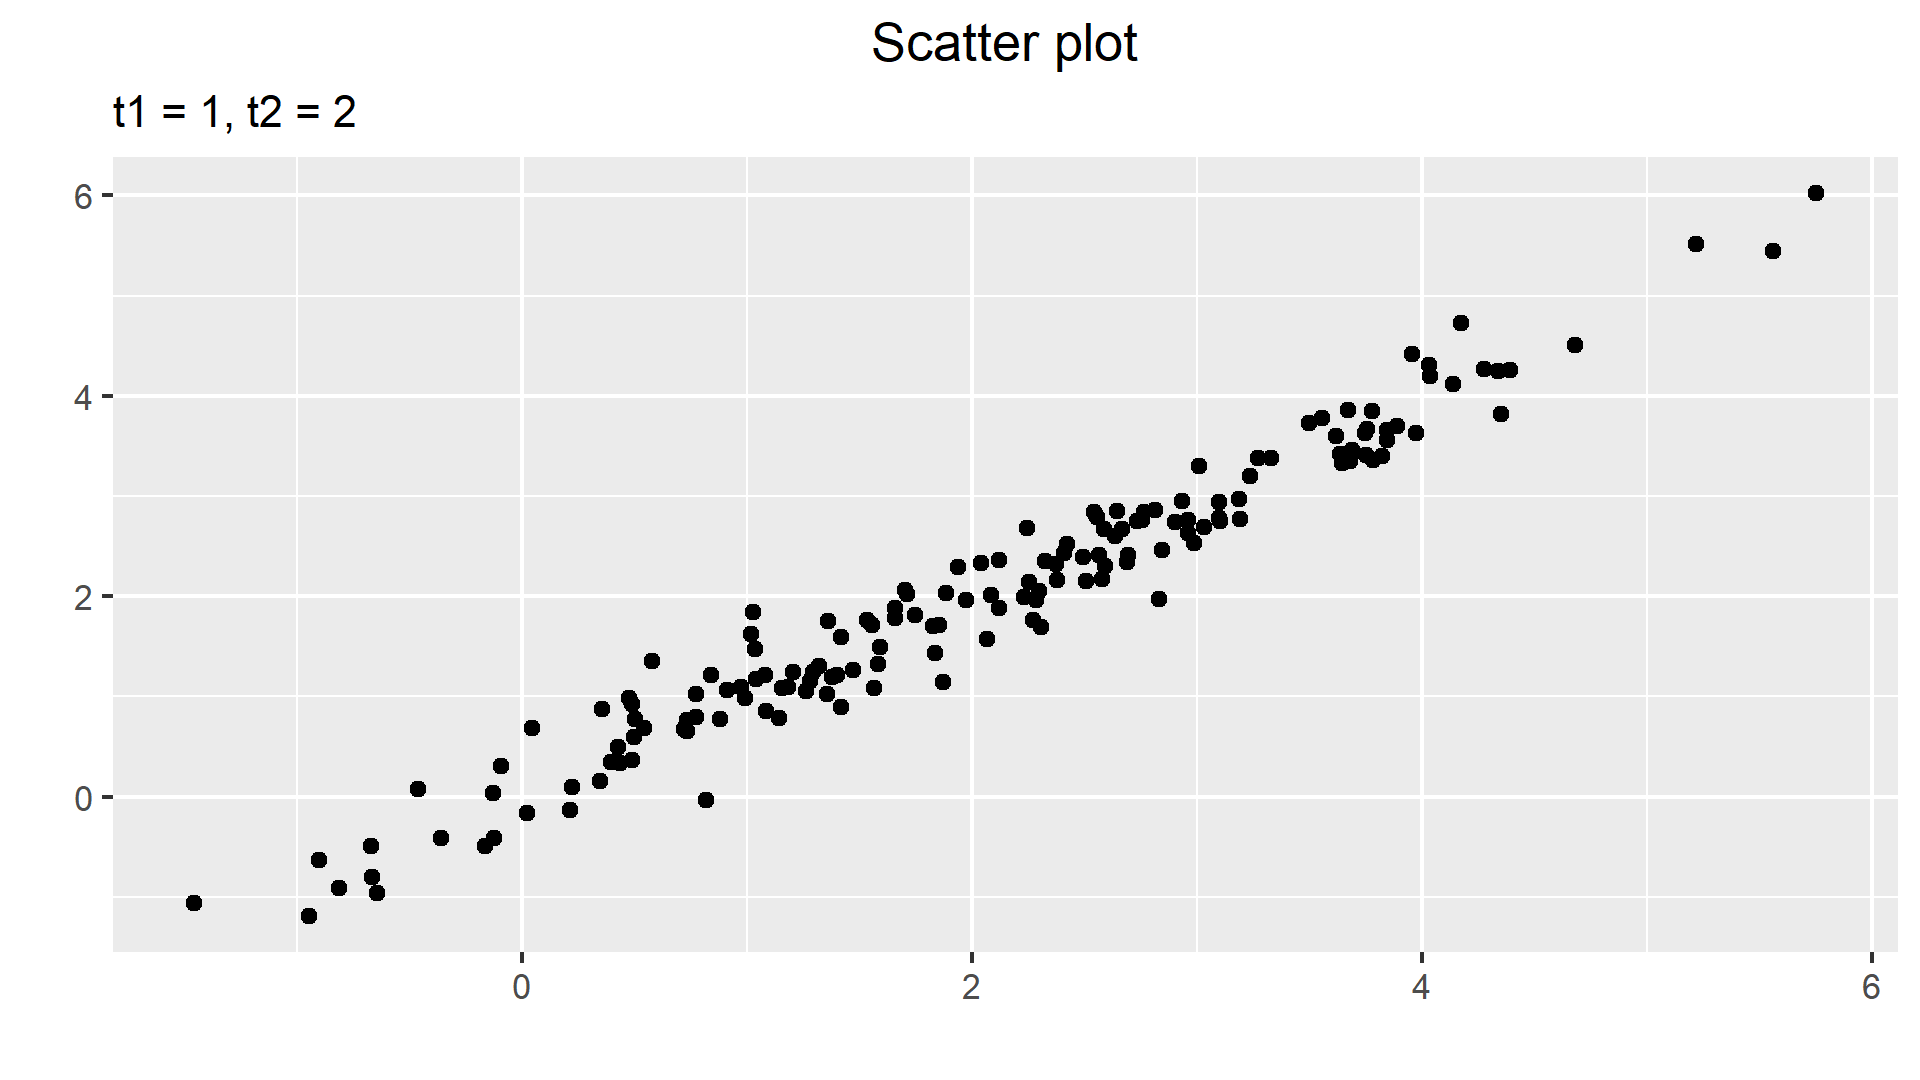
\includegraphics[width=1\linewidth]{../img/1.png}}  \\
	\end{minipage}
\end{figure}

Вычислим выборочный коэффициент $r$ корреляции Пирсона. Согласно формуле:

\begin{equation*}
	r=\frac{\sum_{i=1}^{n}\left(x_{i}-\bar{x}\right)\left(y_{i}-\bar{y}\right)}{\sqrt{\sum_{i=1}^{n}\left(x_{i}-\bar{x}\right)^{2} \sum_{i=1}^{n}\left(y_{i}-\bar{y}\right)^{2}}}
\end{equation*}

В коде это выглядит:

\begin{minted}{R}
> r <- (sum((selected_cut$t1 - mean(selected_cut$t1))*
+              (selected_cut$t2 - mean(selected_cut$t2))))/ 
+   (sqrt(sum((selected_cut$t1 - mean(selected_cut$t1))^2) *
+           sum((selected_cut$t2 - mean(selected_cut$t2))^2)))
> r
[1] 0.9779025
\end{minted}

и занимает 4 строчки. Очевидно, что такого рода вычисления бессмысленно выполнять вручную. 
\pagebreak

Поэтому имеем вместе с доверительными интервалами, формулировкой альтернативной гипотезы и $p-$уровнем значимости для этой гипотезы:
\begin{minted}{R}
> cor_test <- cor.test(selected_cut$t1, selected_cut$t2)
> cor_test

	Pearson`s product-moment correlation
	
	data:  selected_cut$t1 and selected_cut$t2
	t = 58.796, df = 158, p-value < 2.2e-16
	alternative hypothesis: true correlation is not equal to 0
	95 percent confidence interval:
	0.9699081 0.9837906
	sample estimates:
	cor 
	0.9779025
\end{minted}

То есть:
\begin{align*}
	r &= 0.9779025\\
	r_{LB} &= 0.9699081\\
	r_{UB} &= 0.9837906\\
	0.9699081 < &0.9779025 < 0.9837906
\end{align*}

Сравним с истинным значением коэффициента корреляции:
\begin{minted}{R}
> r_tr <- Sigma_mat[1,2]/
+         sqrt(Sigma_mat[1,1] * Sigma_mat[2,2])
> r_tr
[1] 0.9753099
\end{minted}

Истинное значение коэффициента корреляции попадает в доверительный интервал.



\pagebreak
%%%%%%%%%%%%%%%%%%%%%%%%%%%%%%%%%%%%%%%%%%%%%%%%%%%%%%%%%%%%%%%%%%%%%%%%%%%%%%%%%%%%%%%%%%%%%%%%%%%%%%%%%%%%%%%%%%%%%%%%%%%%%%%%%%
\subsubsection*{Второй случай: $t_1 = 20, \; t_2 = 150$}
Получим сечение:

\begin{minted}{R}
> t1 <- 20
> t2 <- 150
> selected_cut <- as.data.frame(matrix(c(sapply(traj_list, `[[`, t1),
+                                        sapply(traj_list, `[[`, t2)),
+                                      ncol = 2, byrow = F))
> colnames(selected_cut) <- c("t1","t2")
> head(selected_cut)
t1          t2
1  4.321029147  2.96629306
2 -0.482835214 -0.17319608
3  1.204216338  3.51484731
4  1.971526428  1.13883326
5  0.007253878  2.03409005
6  1.351975832  0.08824699
\end{minted}

Построим диаграмму рассеяния для полученной пары сечений:

\begin{minted}{R}
> png(filename = "../img/2.png",
+     width = 1920, height = 1080,
+     res = 96 * 3)
> ggplot(selected_cut, aes(x = t1, y = t2)) + geom_point() +
+   labs(title = "Scatter plot",
+        subtitle = "t1 = 1, t2 = 2",
+        x = "", y = "") + 
+   theme(plot.title = element_text(hjust=0.5))
> dev.off()
\end{minted}

\begin{figure}[H]
	\begin{minipage}[h]{1\linewidth}
		\center{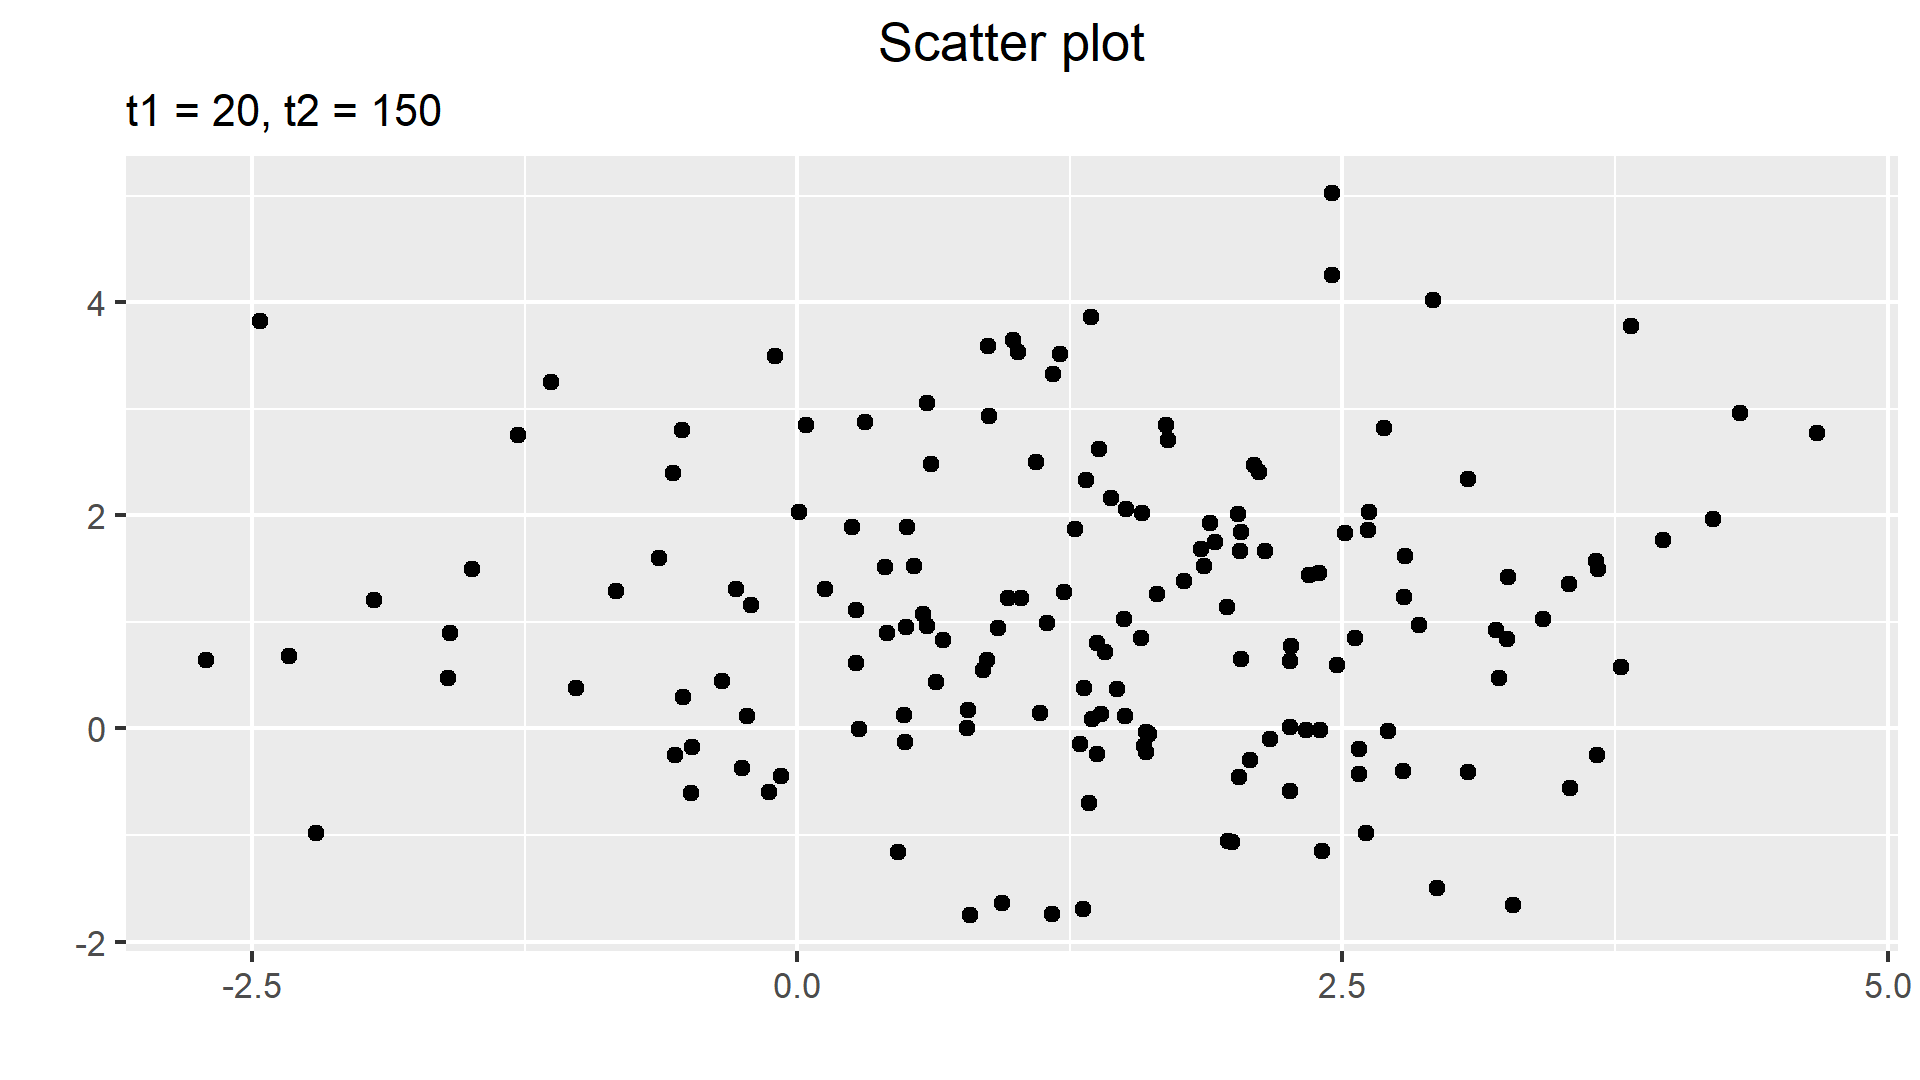
\includegraphics[width=0.85\linewidth]{../img/2.png}}  \\
	\end{minipage}
\end{figure}

\begin{minted}{R}
> cor_test <- cor.test(selected_cut$t1, selected_cut$t2)
> cor_test
	Pearson`s product-moment correlation
	data:  selected_cut$t1 and selected_cut$t2
	t = 0.13647, df = 158, p-value = 0.8916
	alternative hypothesis: true correlation is not equal to 0
	95 percent confidence interval:
	-0.1445461  0.1657357
	sample estimates:
	cor 
	0.01085617 
\end{minted}
\begin{align*}
	r &= 0.01085617 \\
	r_{LB} &= -0.1445461\\
	r_{UB} &= 0.1657357\\
	-0.1445461 < &0.01085617 < 0.1657357
\end{align*}


Сравним с истинным значением коэффициента корреляции:
\begin{minted}{R}
> r_tr <- Sigma_mat[20,150]/
+         sqrt(Sigma_mat[20,20] * Sigma_mat[150,150])
> r_tr
[1] 0.03877421
\end{minted}

Истинное значение коэффициента корреляции попадает в доверительный интервал.





\pagebreak
%%%%%%%%%%%%%%%%%%%%%%%%%%%%%%%%%%%%%%%%%%%%%%%%%%%%%%%%%%%%%%%%%%%%%%%%%%%%%%%%%%%%%%%%%%%%%%%%%%%%%%%%%%%%%%%%%%%%%%%%%%%%%%%%%%
\subsubsection*{Третий случай: $t_1 = 130, \; t_2 = 155$}
Получим сечение:

\begin{minted}{R}
> t1 <- 130
> t2 <- 155
> selected_cut <- as.data.frame(matrix(c(sapply(traj_list, `[[`, t1),
+                                        sapply(traj_list, `[[`, t2)),
+                                      ncol = 2, byrow = F))
> colnames(selected_cut) <- c("t1","t2")
> head(selected_cut)
	t1         t2
1 0.64440246  2.6117555
2 0.89216541 -0.8263974
3 1.44862880  3.2505777
4 0.05134677  0.1976001
5 1.61543339  2.3632578
6 1.44139309  0.9403346
\end{minted}

Построим диаграмму рассеяния для полученной пары сечений:

\begin{minted}{R}
> png(filename = "../img/3.png",
+     width = 1920, height = 1080,
+     res = 96 * 3)
> ggplot(selected_cut, aes(x = t1, y = t2)) + geom_point() +
+   labs(title = "Scatter plot",
+        subtitle = "t1 = 130, t2 = 155",
+        x = "", y = "") + 
+   theme(plot.title = element_text(hjust=0.5))
> dev.off()
\end{minted}

\begin{figure}[H]
	\begin{minipage}[h]{1\linewidth}
		\center{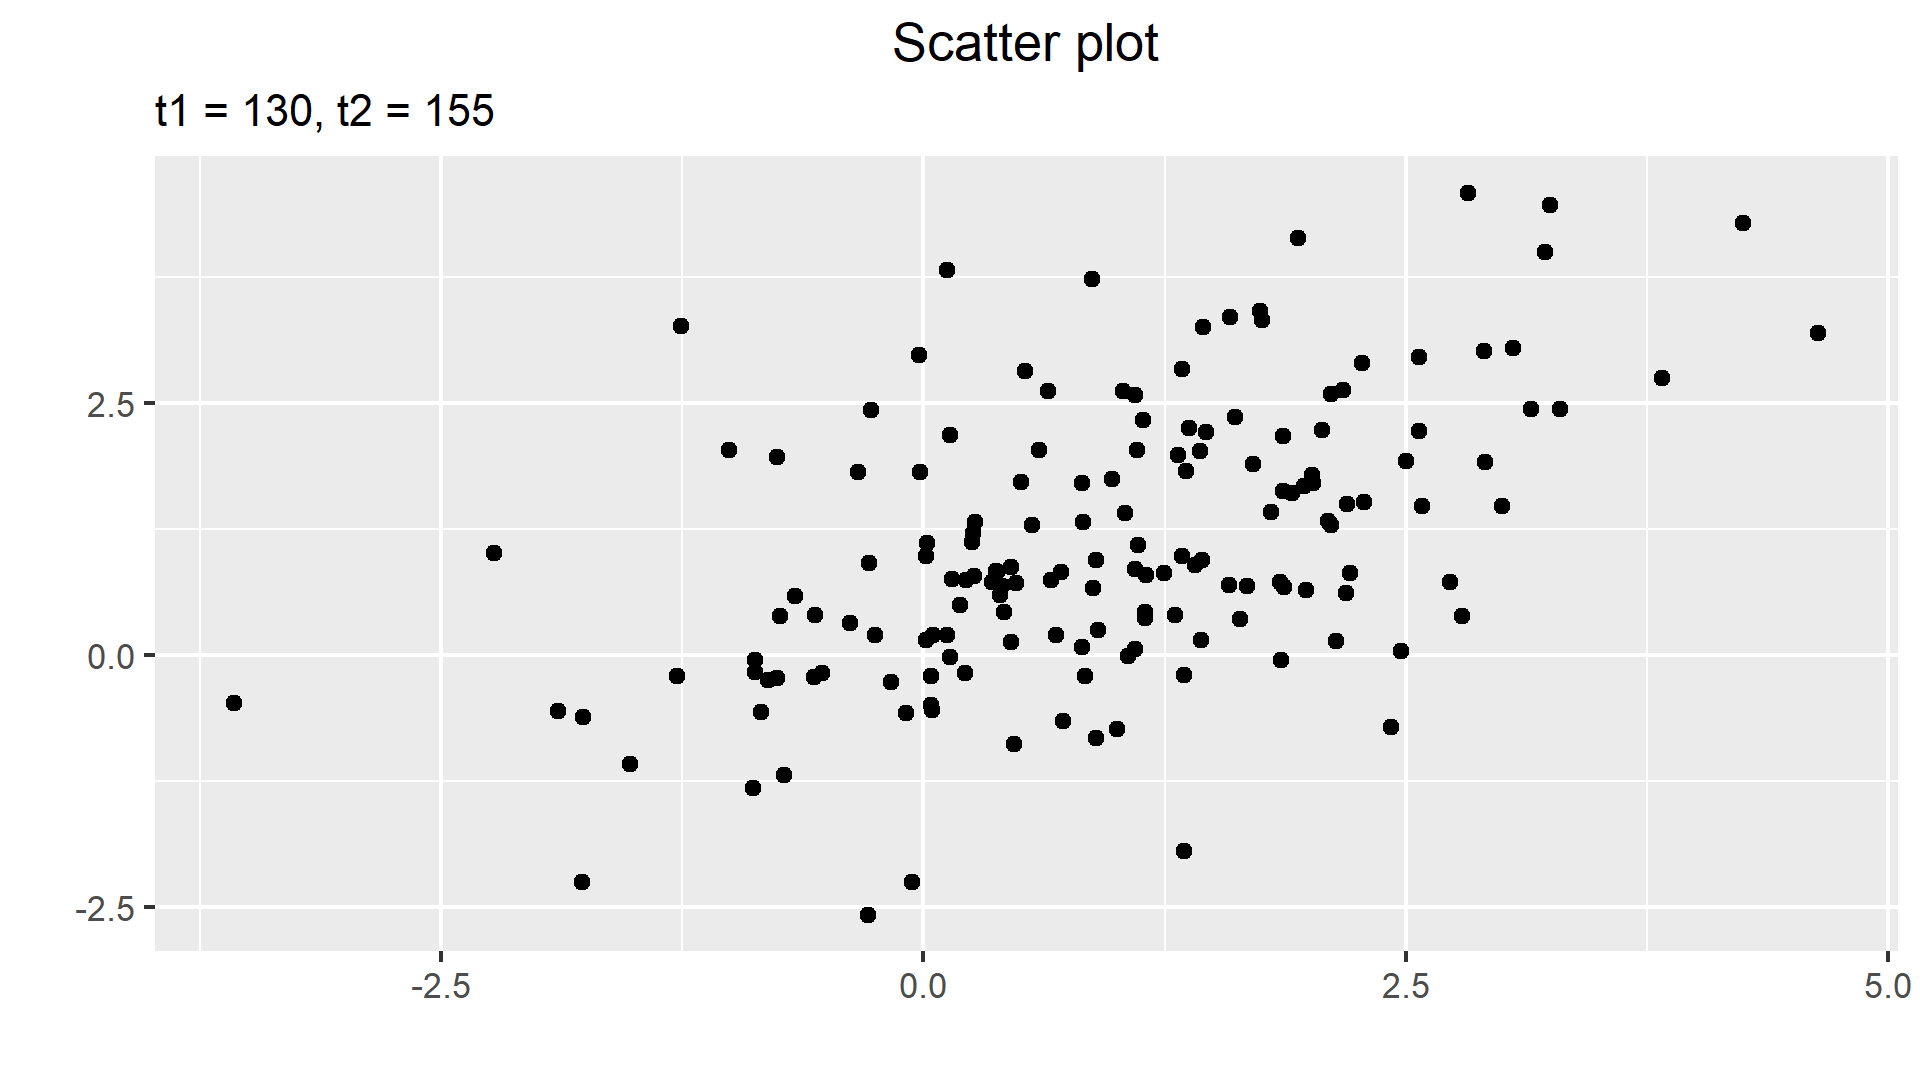
\includegraphics[width=0.85\linewidth]{../img/3.png}}  \\
	\end{minipage}
\end{figure}


\begin{minted}{R}
> cor_test <- cor.test(selected_cut$t1, selected_cut$t2)
> cor_test
	Pearson`s product-moment correlation
	data:  selected_cut$t1 and selected_cut$t2
	t = 7.6924, df = 158, p-value = 1.457e-12
	alternative hypothesis: true correlation is not equal to 0
	95 percent confidence interval:
	0.3991569 0.6264126
	sample estimates:
	cor 
	0.5219876 
\end{minted}

То есть:
\begin{align*}
	r &= 0.5219876 \\
	r_{LB} &= 0.3991569\\
	r_{UB} &= 0.6264126\\
	0.3991569 < &0.5219876 <0.6264126
\end{align*}


\begin{minted}{R}
> r_tr <- Sigma_mat[130,155]/
+         sqrt(Sigma_mat[130,130] * Sigma_mat[155,155])
> r_tr
[1] 0.53526141
\end{minted}

Истинное значение коэффициента корреляции попадает в доверительный интервал.


\pagebreak
\subsection*{Построение коррелограммы}

Рассмотрим корреляционную матрицу по всем парам сечений (округляем до 2 знаков после запятой):

\begin{minted}{R}
> traj_list_tr <- as.data.frame(t(simplify2array(traj_list)))
> M<-round(cor(traj_list_tr),2)
> dim(M)
[1] 201 201
# Верхние 10*10 элементов корреляционой матрицы
> M[1:10,1:10]
     V1   V2   V3   V4   V5   V6   V7   V8   V9  V10
V1  1.00 0.98 0.96 0.94 0.92 0.90 0.87 0.85 0.83 0.80
V2  0.98 1.00 0.98 0.96 0.94 0.92 0.89 0.87 0.85 0.82
V3  0.96 0.98 1.00 0.98 0.96 0.94 0.91 0.89 0.86 0.84
V4  0.94 0.96 0.98 1.00 0.98 0.95 0.93 0.91 0.88 0.85
V5  0.92 0.94 0.96 0.98 1.00 0.97 0.95 0.92 0.90 0.87
V6  0.90 0.92 0.94 0.95 0.97 1.00 0.97 0.95 0.92 0.89
V7  0.87 0.89 0.91 0.93 0.95 0.97 1.00 0.98 0.94 0.91
V8  0.85 0.87 0.89 0.91 0.92 0.95 0.98 1.00 0.97 0.94
V9  0.83 0.85 0.86 0.88 0.90 0.92 0.94 0.97 1.00 0.97
V10 0.80 0.82 0.84 0.85 0.87 0.89 0.91 0.94 0.97 1.00
\end{minted}

Построим коррелограмму наших сечений:

\begin{minted}{R}
> library(corrplot)
> corrplot(M, method="color", tl.pos='n')
\end{minted}

\begin{figure}[H]
	\begin{minipage}[h]{1\linewidth}
		\center{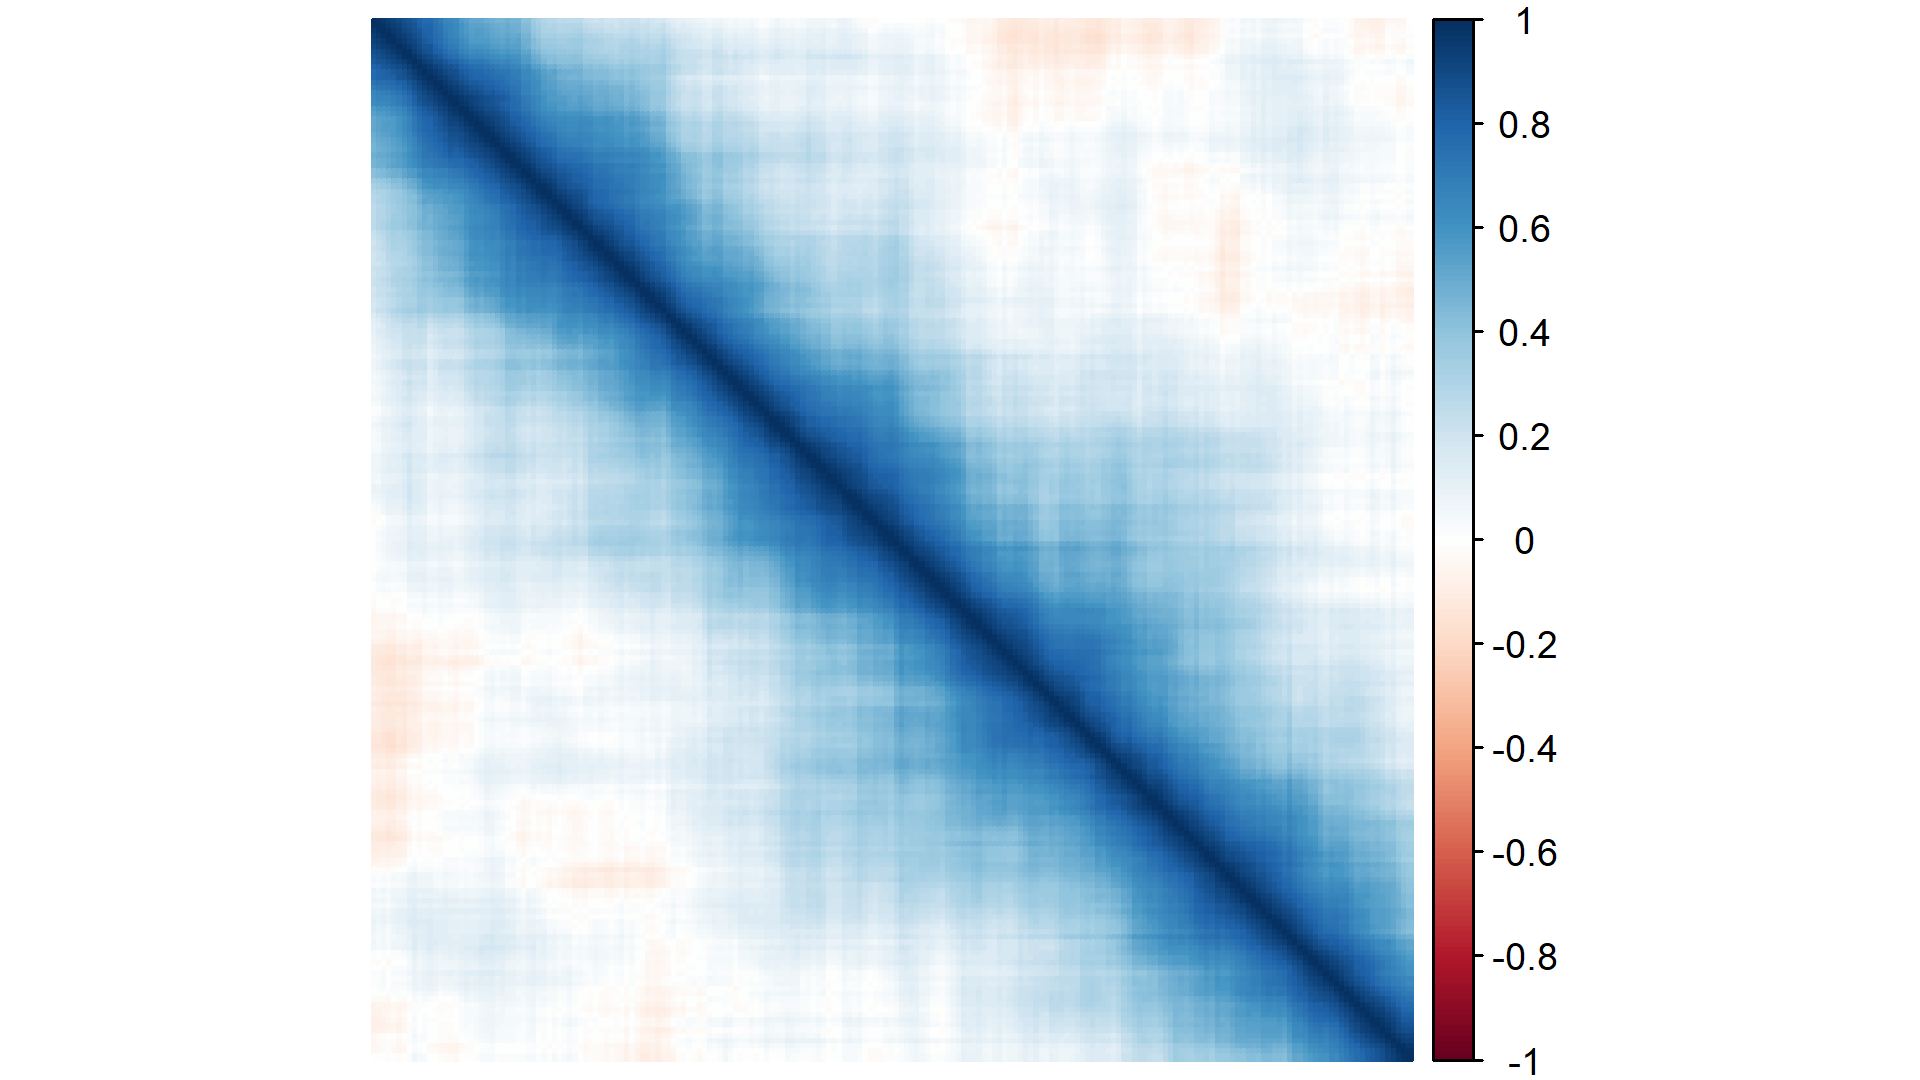
\includegraphics[width=1\linewidth]{../img/corrplot.png}}  \\
		\caption*{Коррелограмма сечений}
	\end{minipage}
\end{figure}


Анализируя полученную диаграмму, делаем вывод о существовании двух принципиальных кластеров: 1) вдоль главной диагонали, 2) вдали от главной диагонали. Им соответствует 3 области на коррелограмме:

\begin{figure}[H]
	\begin{minipage}[h]{1\linewidth}
		\center{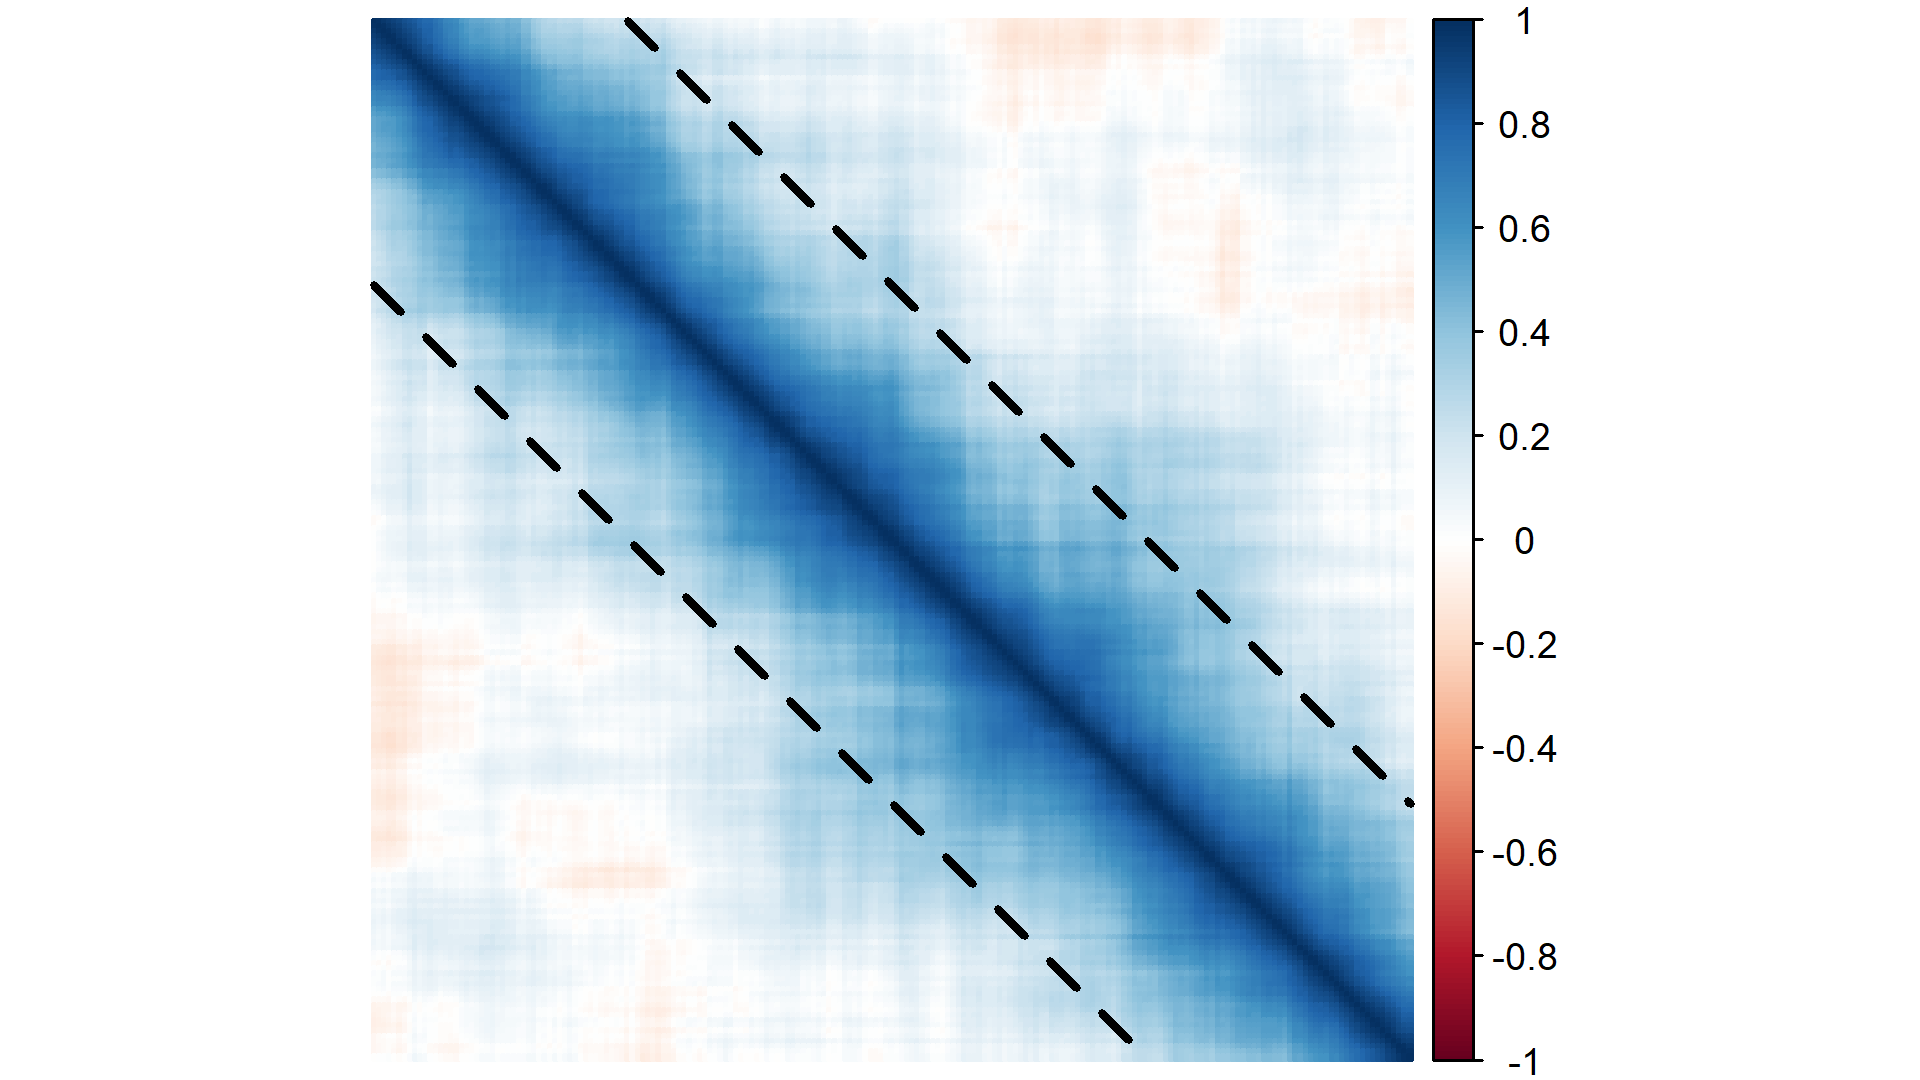
\includegraphics[width=1\linewidth]{../img/corrplot_clustered.png}}  \\
		\caption*{Кластеризованная коррелограмма сечений}
	\end{minipage}
\end{figure}

\pagebreak
Таким образом, можем заключить, что соседние значения $t_1$ и $t_2$ имеют наибольшие коэффициенты корреляции и при удалении друг от друга (при увеличении модуля разности $t_1$ и $t_2$) происходит уменьшение коэффициента корреляции до нуля. Кроме того, можно заметить, что отрицательных значений коэффициента корреляции существенно меньше неотрицательных. Действительно:

\begin{minted}{R}
> M_negative <- length(M[M<0])
> M_negative # Число отрицательных коэффициентов корреляции
[1] 4310
> length(M) # Количество элементов в корреляционной матрице (201*201)
[1] 40401
> M_negative_perc <- M_negative / length(M)
> M_negative_perc # Процент отрицательных элементов
[1] 0.1066805
\end{minted}

\pagebreak
\subsection*{Выводы}
В результате проделанной работы были:
\begin{itemize}
	\item Смоделированы $N=160$ траекторий гауссовского процесса на отрезке $[0;T] = [0;10]$ с заданным математическим ожиданием ${m(t) = 1 + \exp(-t)}$ и заданной автоковариационной функцией $K(t_1,t_2) = 2\exp(-\frac{t_2-t_1}{2})$;
	\item Рассмотрено в ближайшем приближение 3 пары сечений построенного процесса (для близких значений $t_1$ и $t_2$, для далёких, для соседних)
	\item Для рассмотренных пар сечений были:
		\subitem построены диаграммы рассеяния,
		\subitem рассчитаны выборочные коэффициенты корреляции,
		\subitem построены 95\% доверительные интервалы,
		\subitem сделаны выводы относительно принадлежности истинного коэффициента корреляции построенным доверительным интервалам;
	\item Построена и кластеризована коррелограмма сечений
	\item Сделаны выводы относительно зависимости коэффициента корреляции между парами сечений в зависимости от <<удалённости>> между рассматриваемыми парами $t_1$ и $t_2$.
\end{itemize}











\end{document}